
\documentclass{abgabe}
\begin{document}

\begin{questions}
    \qformat{\thequestion. \textbf{\thequestiontitle} \hfill}
    \titledquestion{Softwarekrise}
    Die Softwarekrise wurde als das Problem eingeführt, das mit Softwaretechnik gelöst werden soll. 
    Auch wenn der Begriff aus den 60er Jahren stammt, so ist er auch heute noch anwendbar.
    \begin{parts}
        \part 
        Wählen Sie einen charakteristischen Aspekt der Softwarekrise aus der Vorlesung (oder externen Quellen) und erläutern Sie ihn in eigenen Worten. 
        Zwei Sätze genügen.
        \begin{solution}
            Aus \href{https://en.wikipedia.org/wiki/Software_crisis}{Wikipedia} (und der Vorlesung):
            
            \begin{displayquote}
                Software crisis is a term used in the early days of computing science for the difficulty of writing useful and efficient computer programs in the required time. 
                The software crisis was due to the rapid increases in computer power and the complexity of the problems that could now be tackled. 
                With the increase in the complexity of the software, many software problems arose because existing methods were inadequate.
            \end{displayquote}
        \end{solution}
        
        \part 
        Die Charakterisierung der Softwarekrise spricht verschiedene Ebenen an. 
        Erläutern Sie die Problematik bzgl. \emph{Qualitätssicherung} und \emph{Ökonomie} (Entwicklungsaufwand).
        \begin{solution}
            \emph{Qualitätssicherung}, aus \href{https://en.wikipedia.org/wiki/Softwarequalität}{Wikipedia}:
            
            \begin{displayquote}
                Für die Sicherstellung, dass die Software bezüglich der verschiedenen Qualitätsmerkmale den Anforderungen entspricht (= Qualitätssicherung, kurz QS), existieren verschiedene Vorgehensmodelle und -methoden.
                
                Manche Modelle lassen sich eher dem Konzept der Prozessqualität zuordnen. 
                Dieses geht davon aus, dass ein qualitativ hochwertiger Prozess der Produkterstellung die Entstehung von qualitativ hochwertigen Produkten begünstigt. 
                Deshalb stellen die nachfolgenden Modelle Qualitätsanforderungen an den Prozess, in dem die Software entwickelt wird.
                
                Es existieren allerdings auch Vorgehensmodelle, wie der Goal-Question-Metric-Ansatz, die zu individuellen Qualitätsmodellen führen. 
            \end{displayquote}
            
            \emph{Ökonomie}: minimale Kosten
        \end{solution}
        
        \newpage
        \part 
        Nennen Sie eine Erfahrung, die die Auffassung bestärkt oder widerlegt, dass die Softwarekrise noch anhält. 
        \begin{solution}
            \href{https://xkcd.com/2030/}{xkcd 2030: Voting Software}
            
            \href{https://xkcd.com/2030/}{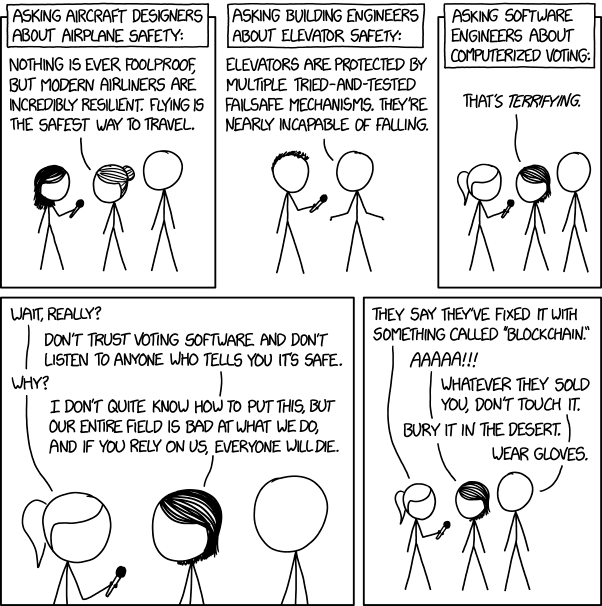
\includegraphics[width=1\textwidth]{voting_software.png}}
        \end{solution}
    \end{parts}
\end{questions}
\end{document}